\icode{E-MV-MU-L3-260625-004}
如图所示的\(xOy\)坐标系中，\(x\)正半轴和\(y\)正半轴上存在两列相干线性平面波波源\(S_1\)、\(S_2\)，传播方向如图。已知直线\(y= x\)上的所有点均为振动减弱点，直线\(y=\frac{3}{4}x\)上距离坐标原点\(O\)最近的加强点\(P\)与\(O\)点的距离为\qty{1}{m}，两平面波的振动周期均为\(T =\)\,\qty{0.5}{s}。下列说法正确的是\paren[]

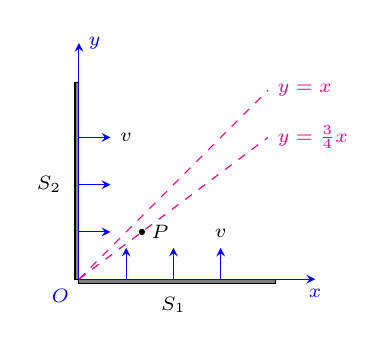
\begin{tikzpicture}[>=stealth,font=\scriptsize]
	\draw[fill=gray] (0,0) rectangle(2.5,-.05) (0,0) rectangle(-.05,2.5);
	\draw[->,blue] (0,0)node[below left]{\(O\)}--(3,0)node[below]{\(x\)};
	\draw[->,blue] (0,0)--(0,3)node[right]{\(y\)};
	\draw[magenta,dashed] (0,0)--(2.4,2.4)node[right]{\(y = x\)} (0,0)--(2.4,1.8)node[right]{\(y = \frac{3}{4}x\)};
	\fill (.8,.6)node[right]{\(P\)} circle(.04);
	\foreach \n in {.6,1.2,1.8}{
		\draw[->,blue] (0,\n)--++(.4,0);
		\draw[->,blue] (\n,0)--++(0,.4);}
	\node at(-.1,1.2)[left]{\(S_2\)};
	\node at(1.2,-.1)[below]{\(S_1\)};
	\node at(.4,1.8)[right]{\(v\)};
	\node at(1.8,.4)[above]{\(v\)};
\end{tikzpicture}
\begin{choices}
	\item 两列波的起振方向相同
	\item 两列波的波速\(v=\)\,\qty{0.8}{m/s}
	\item 直线\(y=\frac{3}{4}x\)上的减弱点距离\(O\)点越远分布越稀疏
	\item 以\(O\)点为圆心、\(5\lambda\)为半径的圆周上有 10 个加强点
\end{choices}
\begin{answer}
	AD
\end{answer}